\documentclass{exam}
\usepackage{graphicx}
\graphicspath{ {images/} }
\usepackage{amsmath}
\usepackage{array}
\usepackage{tabularx}
\usepackage[export]{adjustbox}
\usepackage{pythonhighlight}
\usepackage{listings}
\printanswers
\renewcommand{\solutiontitle}{\noindent\textbf{Resposta:}\par\noindent}
\begin{document}
\begin{center}
\fbox{\fbox{\parbox{5.5in}{\centering
Universidade Federal de Santa Catarina \\ [1ex]
Departamento de Informática e Estatística \\ [1ex]
INE 5426 - Construção de Compiladores \\ [1ex]
Relatório \\ [1ex] 

}}}
\end{center}

\begin{flushleft}
\vspace{5mm}
\makebox[0.542\linewidth]{Nome: Fabio Oliveira de Abreu (18100529)}
\makebox[0.595\linewidth]{Nome: Bruno Duarte Barreto Borges (18100519)}
\makebox[0.52\linewidth]{Nome: Erik Kazuo Sugawara (18100528)}

\vspace{5mm}
\makebox[0.5\linewidth]{Professor: Alvaro Junio Pereira Franco}
\end{flushleft}

% ------  Questions ------
\vspace{5mm}
\begin{questions}
    \question Identificação dos tokens.
        \begin{solution}
            A identificação inicial dos tokens foi retirada da grámatica CC-2021-2,
            onde, para facilitar a organização dentro do código, separamos cada token em cinco grupos:
            palavras reservadas, operadores, símbolos especiais, constantes e identificadores. 
            Seguem alguns exemplos de tokens com a sua expressão regular.
            \begin{python}
t_ASSIGN = r'\='
t_GT = r'\>'
t_LT = r'\<'
t_EQ = r'\=='
t_LE = r'\<='
t_GE = r'\>='
t_NEQ = r'\!='
t_PLUS = r'\+'
t_MULTIPLY = r'\*'
t_DIVIDE = r'\/'
t_REM = r'\%'
            \end{python}

        \end{solution}
    \question Produção das definições regulares para cada token.
        \begin{solution}

            Para produção das definições regulares, foram utilizadas expressões regulares. 
            Como mostrado anteriormente, para definições simples, como os sinais e operadores, 
            foi possível usar a definição em formato de variável. Porém, para definições mais 
            complexas e que necessitavam de tratamento extra, foi necessário usar o formato de função, 
            que também permite o tratamento dos tokens lidos. Segue um exemplo, da definição regular
            do token "FLOAT" utilizando a ferramenta PLY.
            \begin{python}
def t_float_constant(t):
    r'[+-]?\d+\.\d+'
    t.value = float(t.value)
    return t
            \end{python}    
        \end{solution}

    \question Construção dos diagramas de transição para cada token.
        \begin{solution}
            Os diagramas de transição dos tokens foram feitos em uma tabela que se localiza no arquivo TOKENS.xlsx.
            Abaixo, há um exemplo de tabela de transição para um dos tokens identificados (sendo 'digit' a declaração para números de 0 a 9).
            \begin{center}
                \begin{tabular}{|c|c|c|c|}
                \hline
                int\_constant & + & - & digit \\
                \hline
                $\rightarrow$ q0 & q1 & q1 & q2 \\
                \hline
                q1 & - & - & q2  \\ 
                \hline
                *q2 & - & - & q2 \\
                \hline
            \end{tabular}
            \end{center}

        \end{solution}

    \question Descrição de uma tabela de símbolos (como foi implementada),
    quais são os símbolos armazenados na tabela e quais são os atributos dos
    símbolos escolhidos para armazenar na tabela.
        \begin{solution}
            A descrição da tabela de símbolos foi feita através dos tokens que eram retornados pelo analisador léxico,
            onde, dado uma entrada, a ferramenta identificava seu respectivo token. Com todos tokens identificados, é
            utilizado o método "print\_table" que imprime a tabela de forma elegante no próprio terminal. Os atributos
            que foram escolhidos para serem mostrados na tabela foram: Token, Valor, Linha e Coluna.
            \begin{python}
def print_table(lexer):
    pattern = "{:^25} | {:^20} | {:^5} | {:^5}"
    print("\033[4m" + pattern.format("TOKEN", "VALUE", "L", "C") + "\033[0m")
    while True:
        tok = lexer.token()
        if not tok:
            break
        print(pattern.format(tok.type, tok.value, tok.lineno, find_column(tok))) 

    for e in errors:
        print(e)
            \end{python}
        \end{solution}
    \question Se não usou ferramenta, uma descrição da implementação do analisador
     léxico (Usou diagramas de transição? Quais? Quantos? Se não usou
    diagramas de transição, então o que foi usado?)
        \begin{solution}
            Foi utilizado a ferramenta PLY (Python Lex-Yacc).
        \end{solution}

    \question Se usou ferramenta, uma descrição detalhada da entrada exigida
    pela ferramenta e da saída dada por ela. É necessário haver exemplos
    pequenos da entrada e da saída gerada pela ferramenta com essa entrada.
        \begin{solution}
            Para a criação do analisador léxico, foi utilizada o PLY (Python Lex-Yacc),
            uma implementação das ferramentas lex e yacc para python. Nela, podemos
            criar uma lista de tokens a serem identificados pelo analisador, onde devem
            ser armazenados em uma lista chamada "tokens". As váriaveis
            e funções que se iniciam pelos caracteres "t\_" são identificadas como um token
            pelo interpretador, onde podemos definir suas respectivas expressões regulares.
            Executando o PLY em uma string passada, no caso do nosso analisador, obtida de um 
            arquivo cujo caminho é passado como parâmetro 'file' no make, é possível usar o
            método 'token()' para obter o próximo lexema identificado pelo analisador. O método
            retorna um objeto com o token, a string identificada, a linha e a posição léxica 
            (que pode ser usada para calcular a coluna). Com isso podemos construir a tabela
            de símbolos referente ao arquivo passado.

        \end{solution}
       
            \begin{center}
            \begin{lstlisting}[language=bash]
             $ make run file='tmp/lil_example.lcc'
            \end{lstlisting}
            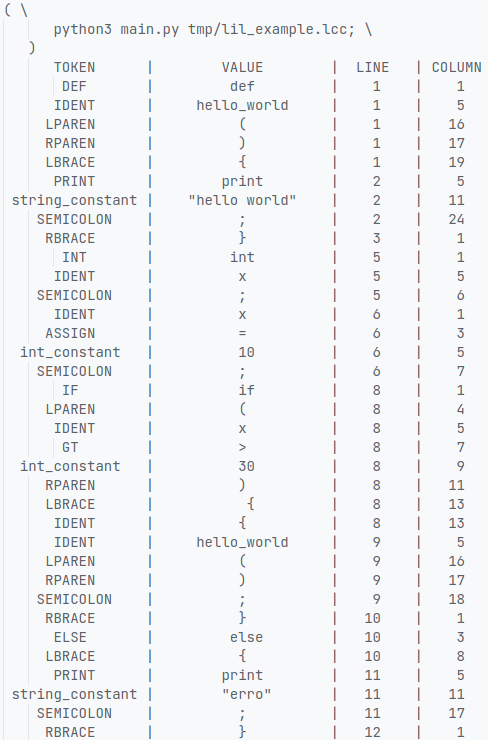
\includegraphics[height=17cm,width=16cm,keepaspectratio]{example.png}
            \end{center}
\end{questions}
\end{document}
